% Created 2023-02-28 Tue 12:32
% Intended LaTeX compiler: pdflatex
\documentclass[presentation]{beamer}
\usepackage[utf8]{inputenc}
\usepackage[T1]{fontenc}
\usepackage{graphicx}
\usepackage{longtable}
\usepackage{wrapfig}
\usepackage{rotating}
\usepackage[normalem]{ulem}
\usepackage{amsmath}
\usepackage{amssymb}
\usepackage{capt-of}
\usepackage{hyperref}
\usetheme[progressbar=foot]{metropolis}
\usetheme{metropolis}
\usecolortheme{}
\usefonttheme{}
\useinnertheme{}
\useoutertheme{}
\author{Andrew Jensen}
\date{March 9, 2023}
\title{Joint Track Machine Learning}
\hypersetup{
 pdfauthor={Andrew Jensen},
 pdftitle={Joint Track Machine Learning},
 pdfkeywords={},
 pdfsubject={},
 pdfcreator={Emacs 28.1 (Org mode 9.6)}, 
 pdflang={English}}
\usepackage{biblatex}
\addbibresource{/home/andrew/repo/lit-review/src/myBib.bib}
\addbibresource{~/org/biblio.bib}
\begin{document}

\maketitle
\begin{frame}{Outline}
\tableofcontents
\end{frame}


\section{Introduction}
\label{sec:org4ab3566}
\begin{frame}[label={sec:org02e632a}]{Two columns}
\begin{columns}
\begin{column}{0.4\columnwidth}
\begin{itemize}
\item this slide consists of two columns
\item the first (left) column has no heading and consists of text
\item the second (right) column has an image and is enclosed in an
@example@ block
\end{itemize}
\end{column}
\begin{column}{0.6\columnwidth}
\begin{center}
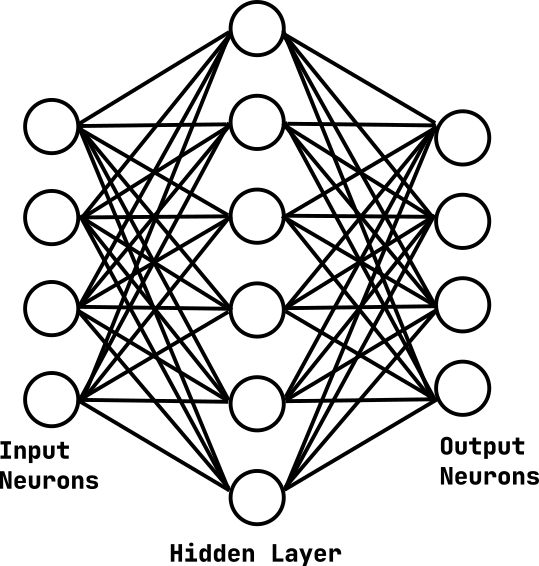
\includegraphics[width=\textwidth]{/home/andrew/repo/lit-review/figures/raster/fcn.png}
\end{center}
\end{column}
\end{columns}
\end{frame}
\begin{frame}[label={sec:orgfda485a}]{Another frame here}
Typing some things here that relate to the research.

\begin{equation*}
  T = F(s,\theta)
\end{equation*}
\end{frame}

\section{Motivation}
\label{sec:orgca6f5e1}
\begin{frame}[label={sec:org3ac28ad}]{The Problem}
\begin{columns}
\begin{column}{0.5\columnwidth}
\begin{itemize}
\item Joints manifest pain during dynamic activity.
\item 20\% of patients receiving TKA are dissatisfied.
\begin{itemize}
\item Instability, pain, unnatural\autocites{bakerRolePainFunction2007}[][]{bournePatientSatisfactionTotal2010}[][]{scottPredictingDissatisfactionFollowing2010}.
\end{itemize}
\item No reliable method of clinically assessing and quantifying joint dynamics.
\end{itemize}
\end{column}
\begin{column}{0.4\columnwidth}
\begin{center}
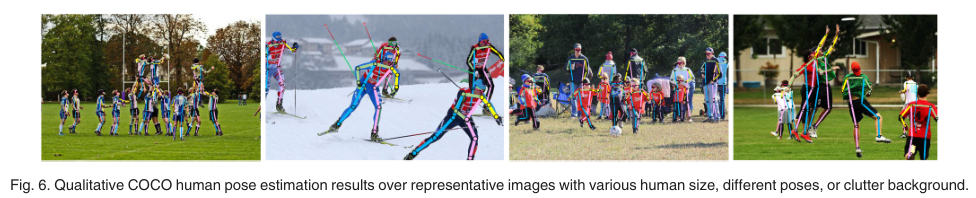
\includegraphics[width=.9\linewidth]{/home/andrew/repo/lit-review/figures/raster/hrnet-human-pose.png}
\end{center}
\end{column}
\end{columns}
\end{frame}
\section{References}
\label{sec:orgd33c319}
\begin{frame}[label={sec:orgbf2c20e},fragile, allowframebreaks, label=]{References}
\AtNextBibliography{\tiny}
\printbibliography
\end{frame}
\end{document}